\section{Metropolis-Hastings \\MCMC (nonlinear model)}

Use the same Metropolis Hastings code to fit the data from gaussfit data.npz to the gaussian function
\begin{equation}
    f(\Vec{x}|\Vec{a})=a_0+a_1e^{-\frac{1}{2}(\frac{x-a_2}{a_3})^2}
\end{equation}

Overplot the joint 68.3\% and 95\% confidence intervals for all combinations of parameters.

\begin{figure*}
    \centering
    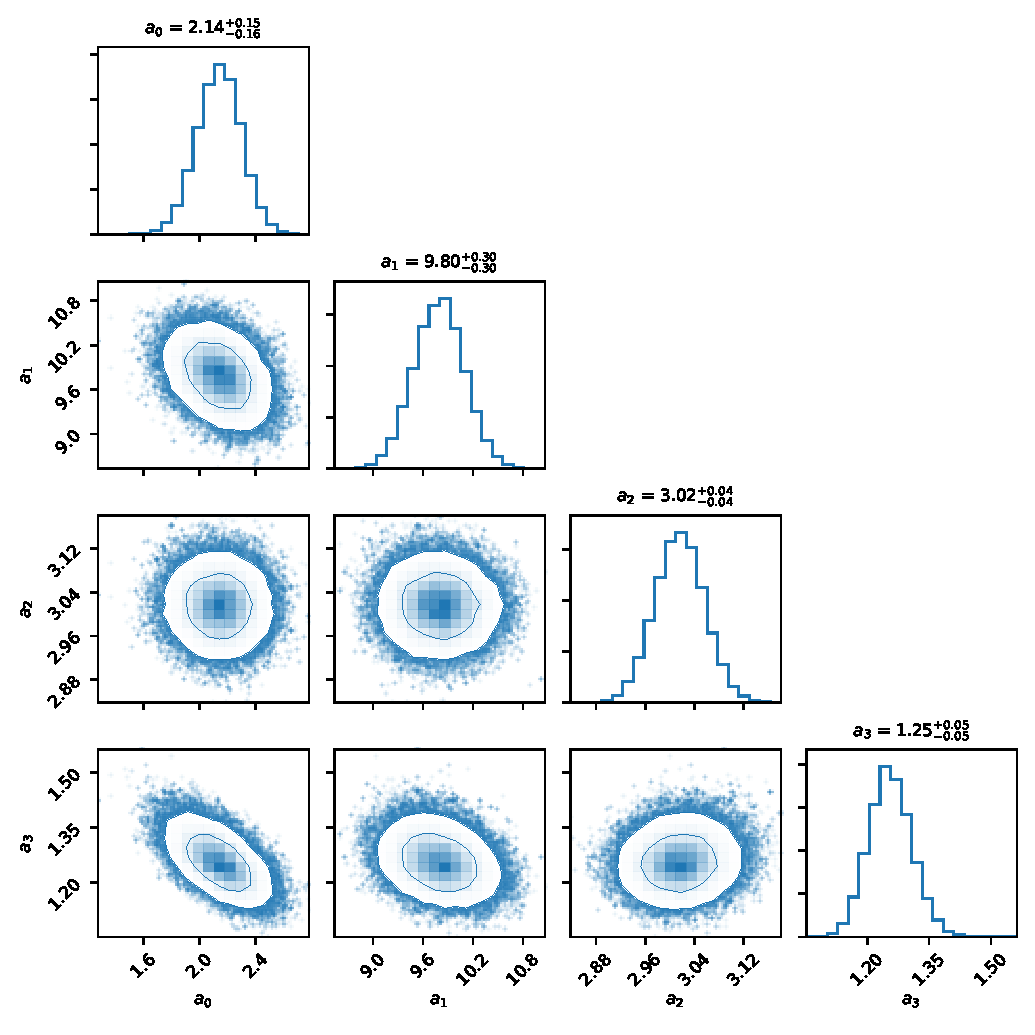
\includegraphics{CodeAndFigures/GaussianModelMetropolisHastings.pdf}
    \caption{Caption}
    \label{fig:GaussHastings}
\end{figure*}